\documentclass[12pt, letterpaper]{article}
\usepackage{graphicx} % Required for inserting images
\usepackage{hyperref}
\usepackage{listings}
\usepackage{amssymb}
\usepackage{amsmath}
\usepackage[english]{babel}
\usepackage{nicefrac, xfrac}
\usepackage{mathtools}
\usepackage[table,xcdraw]{xcolor}
\definecolor{light-gray}{gray}{0.95}
\definecolor{sap}{RGB}{130, 36, 51}
\definecolor{lg}{RGB}{102, 161, 95}
\usepackage[paper=a4paper,left=20mm,right=20mm,bottom=25mm,top=25mm]{geometry}
\newcommand{\code}[1]{\colorbox{light-gray}{\texttt{#1}}}
\newcommand{\codee}[1]{\colorbox{white}{\texttt{#1}}}
\newcommand{\acc}{\\\hphantom{}\\}
\newcommand{\dete}{{\rightarrow}}
\newcommand{\fdot}{{\(\bullet\) }}
\newcommand{\boxedMath}[1]{\begin{tabular}{|c|}\hline \texttt{#1} \\ \hline\end{tabular} :}
\title{Sistemi Operativi 2}
\author{Marco Casu}
\date{\vspace{-5ex}}
\begin{document}



\maketitle
\begin{figure}[h]
    \centering{
    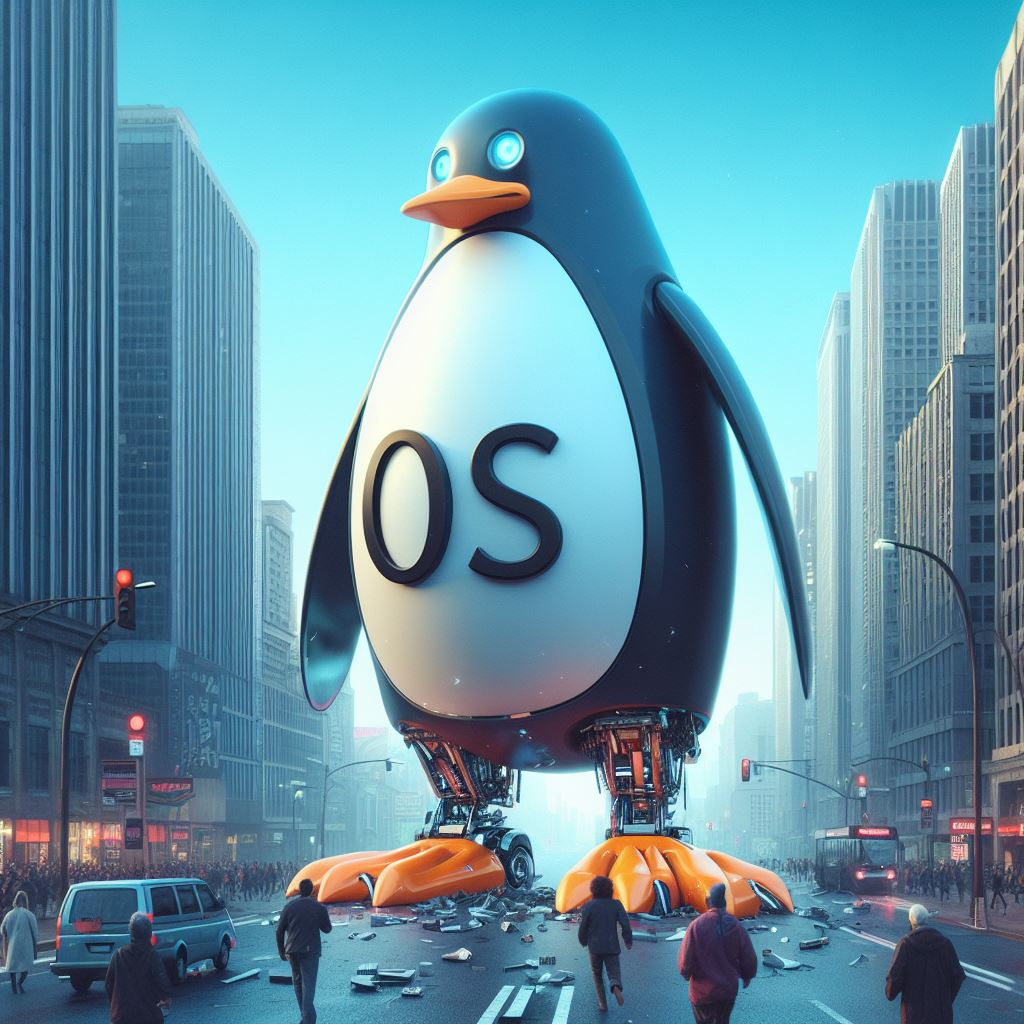
\includegraphics[width=1\textwidth ]{images/cop.jpg}
    }
\end{figure}
\newpage 
\tableofcontents
\newpage
\section{Introduzione}
Ciao
\end{document}
